% Section content template for individual Educative lessons
% This file contains the actual content for a specific section
% Generated from Educative API section content

% Section: Generalization
% Section ID: 4506169807601664
% Section Slug: generalization
% Generated: 2025-12-16T12:49:37.129907

\textbf{Generalization} is a fundamental concept in object-oriented design (OOD) that involves extracting common properties and behaviors from multiple classes and consolidating them into a single parent class. This allows subclasses to inherit shared attributes and methods while having the flexibility to specialize further. Abstracting common behaviors into a parent class simplifies code maintenance, enhances reusability, and supports easier code extension.

\subsection{Importance of generalization}\label{vBz0oRqXV9fqOR3yeJXZ6}

\begin{itemize}
\item
\protect\phantomsection\label{1jFOB-izxWkOnoVcTp9UQ}
\textbf{Code reusability:} Reduces duplication by allowing subclasses to reuse code from the parent class.
\item
\protect\phantomsection\label{yAmoJUtxOgIUwoNV2cq8c}
\textbf{Extensibility:} New classes can easily be added by extending the parent class, without altering existing code.
\item
\protect\phantomsection\label{19WS0Z5t45PZMVVC_zP-h}
\textbf{Polymorphism:} Parent class references can point to child class objects, promoting more general and adaptable code that can easily work with new subclasses in the future.
\item
\protect\phantomsection\label{PLjvNvmbOhOtcjpsNsXwO}
\textbf{Maintainability:} Changes to shared behavior must only be made in one place, making the system easier to manage and less error-prone.
\end{itemize}

\subsection{Generalization vs. specialization}\label{y066UwXA0-HkM2yhsb61q}
\\
Understanding the distinction between generalization and specialization is key to effective object-oriented design:

\begin{itemize}
\item
\protect\phantomsection\label{8U5J3o6JVX9QfB9TyvID7}
\textbf{Generalization:}~Finding common characteristics in different classes and abstracting them into a parent class.
\item
\protect\phantomsection\label{C7Q2AXYv2een_q7TlvivV}
\textbf{Specialization:}~Creating subclasses that define more specific behaviors or attributes.
\end{itemize}
\\
For example, \texttt{Bird} could be a generalized class with common behavior for all birds. We could then specialize this further into \texttt{Sparrow} and \texttt{Eagle} classes, each with additional behaviors unique to those birds.

\begin{figure}[htbp]
 \centering
 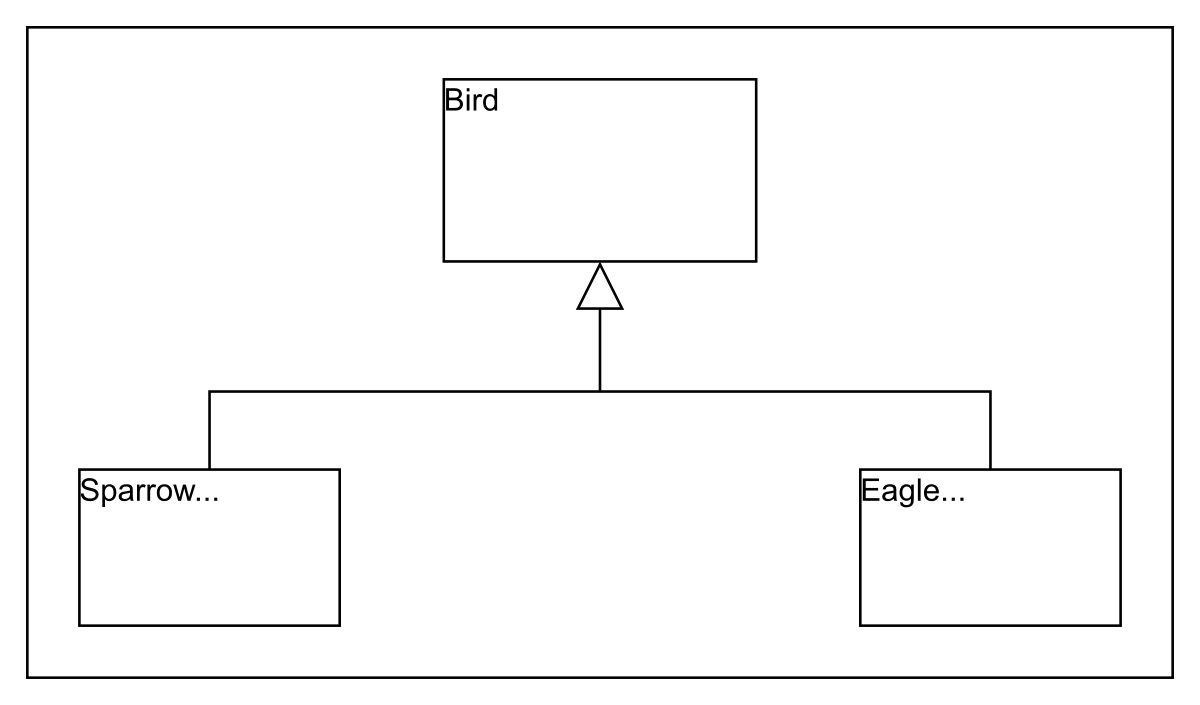
\includegraphics[width=0.5\textwidth]{Images/chapter_2/section_4506169807601664/5253963812044800.png}
 
\end{figure}

\subsection{Generalization and inheritance}\label{wKRpmcqdBlP2SeiSCkqd9}
\\
Generalization is implemented through \textbf{inheritance}, where a child class inherits common properties from the parent class.
\\
In the code below, \texttt{Dog} and \texttt{Cat} inherit \texttt{Animal}'s common behavior and also add their specific features.

\textbf{Generalization and inheritance}

\begin{lstlisting}[language=Java]
// Parent Class: Animal
class Animal {
    public void sleep() {
        System.out.println("Animal is sleeping");
    }

    public void eat() {
        System.out.println("Animal is eating");
    }
}

// Specialized Classes: Dog and Cat
class Dog extends Animal {
    public void bark() {
        System.out.println("The dog barks");
    }
}

class Cat extends Animal {
    public void meow() {
        System.out.println("The cat meows");
    }
}

// Driver code
public class Main {
    public static void main(String[] args) {
        Dog dog = new Dog();
        dog.sleep();  // Inherited method
        dog.bark();   // Dog-specific method
        dog.eat();    // Inherited method

        Cat cat = new Cat();
        cat.sleep();  // Inherited method
        cat.meow();   // Cat-specific method
        cat.eat();    // Inherited method
    }
}
\end{lstlisting}

In the example above:

\begin{itemize}
\item
\protect\phantomsection\label{84jMVL1eaKJzfuuNAooUd}
The \texttt{Animal} class is generalized with common methods \texttt{sleep()} and \texttt{eat()}.
\item
\protect\phantomsection\label{aY2j45-FTHSCr7hndQgo6}
\texttt{Dog} and \texttt{Cat} are specialized classes that inherit the \texttt{sleep()} and \texttt{eat()} methods and add their own unique behavior (\texttt{bark()} and \texttt{meow()}).
\end{itemize}
\\
Instead of repeating \texttt{sleep()} and \texttt{eat()} methods in both \texttt{Dog} and \texttt{Cat}, we've moved them to the \texttt{Animal} class. This allows both \texttt{Dog} and \texttt{Cat} to automatically inherit these behaviors.

\subsection{Generalization and polymorphism}\label{yrY_vvs65DdO2TfeNkw20}
\\
Polymorphism is one of the key benefits of generalization. It allows objects of different subclasses to be treated as objects of the parent class, promoting flexibility and reducing the need for type checking.
\\
We can use polymorphism to refer to an object of type \texttt{Circle} or \texttt{Rectangle} as a \texttt{Shape}. This is achieved because both \texttt{Circle} and \texttt{Rectangle} inherit from \texttt{Shape}.

\textbf{Generalization and polymorphism}

\begin{lstlisting}[language=Java]
// Abstract Parent Class: Shape
abstract class Shape {
    String color;

    Shape(String color) {
        this.color = color;
    }

    // Abstract method (no body)
    abstract double area();
}

// Specialized Class: Circle
class Circle extends Shape {
    double radius;

    Circle(String color, double radius) {
        super(color);
        this.radius = radius;
    }

    @Override
    double area() {
        return Math.PI * radius * radius;
    }
}

// Specialized Class: Rectangle
class Rectangle extends Shape {
    double length, width;

    Rectangle(String color, double length, double width) {
        super(color);
        this.length = length;
        this.width = width;
    }

    @Override
    double area() {
        return length * width;
    }
}

// Driver code
class TestPolymorphism {
    public static void main(String[] args) {
        Shape myShape = new Circle("Red", 5.0); // Circle is treated as Shape
        System.out.println("Circle color: " + myShape.color);
        System.out.println("Circle area: " + myShape.area());

        myShape = new Rectangle("Blue", 4.0, 6.0); // Rectangle is treated as Shape
        System.out.println("Rectangle color: " + myShape.color);
        System.out.println("Rectangle area: " + myShape.area());
    }
}
\end{lstlisting}

In this case, the same \texttt{myShape} reference is used to refer to both \texttt{Circle} and \texttt{Rectangle} objects, demonstrating polymorphism.

\subsection{Generalization in real-world example}\label{wHRMW5cgppc-4BkW8nDJH}
\\
Imagine you are developing a vehicle management system for a logistics company. Many types of vehicles share common features, but there are also subcategories within them.

\begin{figure}[htbp]
 \centering
 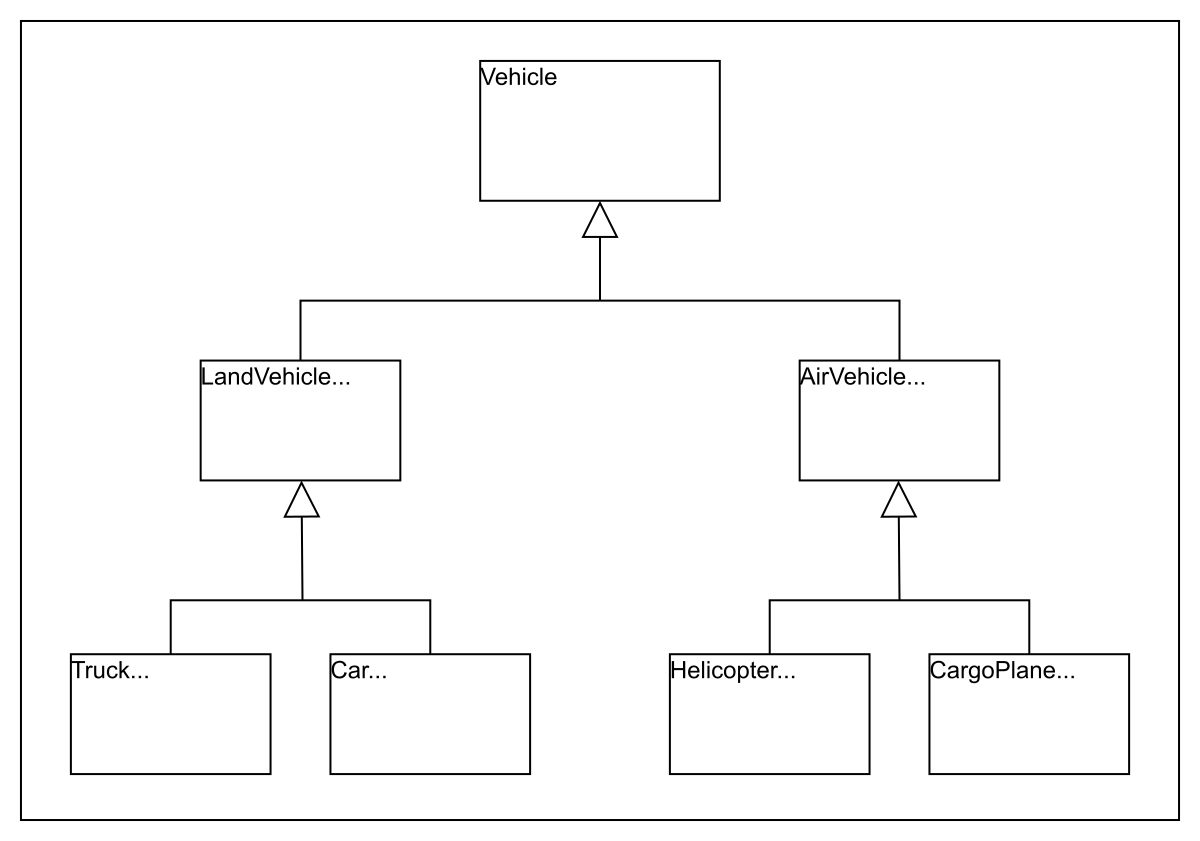
\includegraphics[width=0.5\textwidth]{Images/chapter_2/section_4506169807601664/6605887077482496.png}
 
\end{figure}

At the top level, \texttt{Vehicle} is the parent class, containing shared properties such as \texttt{registrationNumber}, \texttt{capacity}, and a method like \texttt{move()}. This generalizes into two subclasses: \texttt{LandVehicle} and \texttt{AirVehicle}, each inheriting the core features from \texttt{Vehicle} while adding more specific properties relevant to their type.

\begin{itemize}
\item
\protect\phantomsection\label{CCJM3qfk2eCuT4qhqIela}
\texttt{LandVehicle} is further specialized into \texttt{Truck} and \texttt{Car}:

\begin{itemize}
\item
\texttt{Truck} might introduce attributes like \texttt{loadType}.
\item
\texttt{Car} could have properties such as \texttt{passengerCount}.
\end{itemize}
\item
\protect\phantomsection\label{GgIPtNYGHhcxNSDYRtEVz}
\texttt{AirVehicle} is further specialized into \texttt{Helicopter} and \texttt{CargoPlane}:

\begin{itemize}
\item
\texttt{Helicopter} might have features like \texttt{rotorCount}.
\item
\texttt{CargoPlane} could include attributes such as \texttt{maxAltitude} and \texttt{cargoVolume}.
\end{itemize}
\end{itemize}

\subsection{Generalization and the open/closed principle (OCP)}\label{6vWIIzeWRyILS02hSeK1h}
\\
The open/closed principle (part of SOLID principles) states that classes should be \textbf{open for extension} but \textbf{closed for modification}. Generalization helps achieve this by allowing new subclasses to be added without altering the existing code.
\\
Let's say we want to add a new land vehicle type \texttt{Bike}. We create a \texttt{Bike} class that extends \texttt{LandVehicle}.

\begin{figure}[htbp]
 \centering
 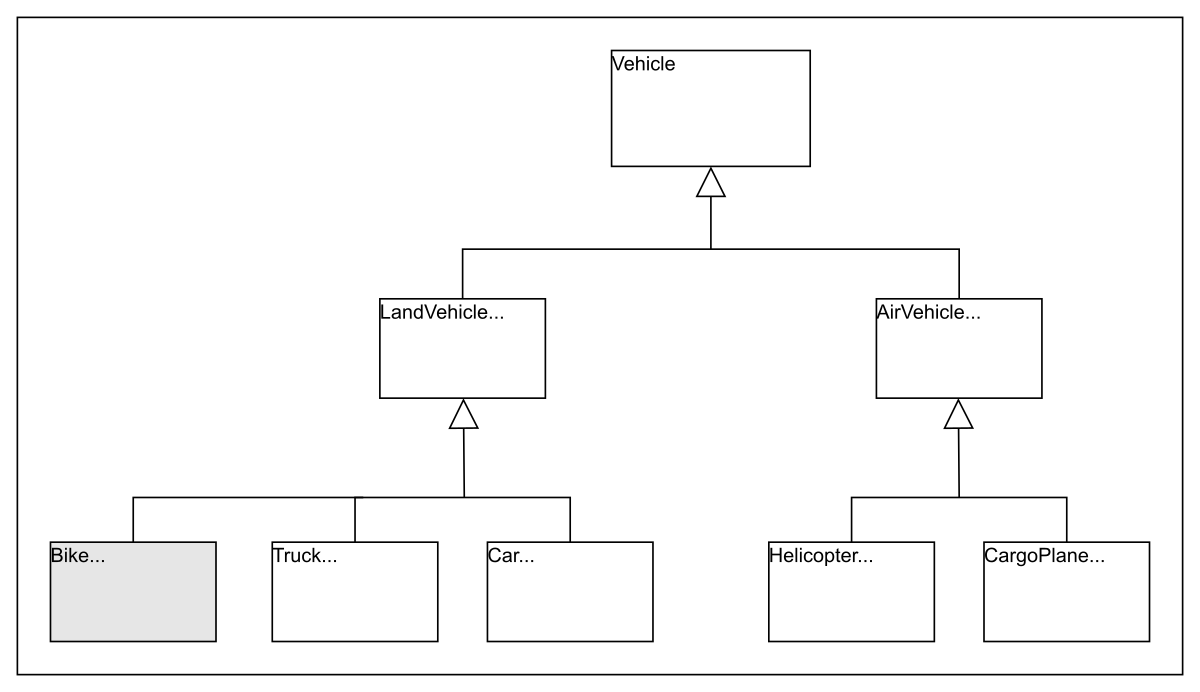
\includegraphics[width=0.5\textwidth]{Images/chapter_2/section_4506169807601664/4575334799114240.png}
 
\end{figure}

We do not need to modify \texttt{Vehicle}, \texttt{LandVehicle}, or any of the existing vehicle classes to add this new type.

% End of section content